\newpage
\section{ Теоретические основы }

\subfile{src/common_definitions}
\subfile{src/common_using_symbol}

\subsection{ Физические процессы в шаговом двигателе }
Если не учитывать насыщение магнитной системы, то справедливо равенство \cite[стр. 82]{Chilikin}:

\begin{equation}
\label{step_motor_torque_common}
    M(\theta)
    = \frac{dW_r}{d\theta_m}
    = p \frac{dW_s}{d\theta}
    = \frac{1}{2} p I_s \frac{dL_s}{d\theta}
        + \frac{1}{2} p I_r \frac{dL_r}{d\theta}
        + \frac{1}{2} p I_{s} I_r \frac{dL_{sr}}{d\theta}
\end{equation}

$I_{s}, I_{r}$ - установившееся значение токов статора и ротора соответсвенно

$L_{s}(\theta)$ - индуктивность статора

$L_{r}(\theta)$ - индуктивность ротора

$L_{sr}(\theta)$ - взаимоиндукция ротора и статора

Частота собственных упругих колебаний ротора \cite[гл 3.1]{Chilikin} при малых отклонениях от положения устойчивого
положения позволяет получить сторогую оценку механической подвижности системы и является ее мерой.

\begin{equation}
\label{step_motor_torque_without_load_and_with_unstable_rotor}
    M(\theta)
    = - M_{m} \sin{\theta}
    = - M_{m} \sin{p\theta_{M}}
\end{equation}

\begin{equation}
\label{step_motor_dynamic_move_equation}
    J \ddot{ \theta_{M} } + M_{m} \sin{p \theta_{M}} = 0
\end{equation}

При малых отклонениях от положения равновесия таких что:
\begin{equation}
    \sin{\theta} \thickapprox 0
\end{equation}

\begin{equation}
    \label{rotor_like_harmonical_oscilator_equation}
    \ddot{\theta} + \frac{p M_{m}}{J} \theta = 0
\end{equation}

\begin{equation}
    \label{friquent_for_rotor_self_oscilating}
    \omega = \sqrt{ \frac{p M_{m}}{J} }
\end{equation}

Процесс изменения тока в обмотке шагового двигателя при ШИМ-управлении \cite[гл. 6.4, стр. 239]{Chilikin}:

Для случая $0 \le \varepsilon \le \zeta$:
\begin{equation}
    \label{winding_current_with_pwm_control_1}
    i[ n; \varepsilon ] = \frac{ U_1 }{ R }
                            \cdot \{ 1
                                     - \frac { e^{ -\sigma \cdot \varepsilon } } { 1 - e^{-\sigma} }
                                            \cdot [ (1 - e^{-n\sigma})
                                                    - e^{ -(1 - \zeta) \cdot \sigma }
                                                        \cdot ( 1 - e^{-n\sigma + \sigma} )
                                                  ]
                                  \}
                        - \frac{ U_2 }{ R }
                            \cdot \frac {e^{-\sigma}} {1 - e^{-\sigma}}
                            \cdot ( 1 - e^{ -n \cdot \sigma + \sigma } )
                            \cdot ( 1 - e^{ -\sigma + \sigma \cdot \zeta } )
\end{equation}

Для случая $\zeta \le \varepsilon \le 1$:
\begin{equation}
    \label{winding_current_with_pwm_control_0}
    i[n; \varepsilon] =
        \frac{ U_{1} + U_{2} }{ R }
            \cdot \frac{ 1 }{ 1 - e^{-\sigma} }
            \cdot (1 - e^{-\sigma\zeta})
            \cdot (1 - e^{-n\sigma})e^{-\sigma\varepsilon + \sigma\zeta}
        - \frac{ U_{2} }{ R }
            \cdot [ 1 - e^{ -( n - 1 + \varepsilon - \zeta ) \sigma } ]
\end{equation}

$\varepsilon = \frac{ t }{ T_\text{ШИМ} }$

$\zeta = \frac{ t_{1} }{ T_\text{ШИМ} }$

$\sigma = \frac{ T }{ T_\text{ШИМ} }$

$T = \frac{ L }{ R }$

$n$ - число периодов импульсов напряжения

$t_{1}$ - время подачи напряжения внутри импульса, с

$T_\text{ШИМ}$ - период ШИМ, с

$t$ - текущее время, с

Максимальное значение тока в импульсе ШИМ согласно (\ref{winding_current_with_pwm_control_1}) при
$\varepsilon=\zeta$ и $U_{2}=0$:

\begin{equation}
    \label{max_current_in_the_n_pwm_pulse}
    i_{max}[n; \zeta] =
        I_{0}
            \cdot \{ 1
                     - \frac{ e^{-\sigma \cdot \zeta} }{ 1 - e^{-\sigma} }
                       \cdot [ (1 - e^{-n\sigma})
                               - e^{ -(1 - \zeta) \cdot \sigma }
                                    \cdot ( 1 - e^{-n\sigma + \sigma} )
                             ]
                  \}
\end{equation}

Где $I_0 = \frac{ U_{1} }{ R }$

Минимальное значение тока в импульсе ШИМ согласно (\ref{winding_current_with_pwm_control_1}) при
$\varepsilon=1$ и $U_{2}=0$:

\begin{equation}
    \label{min_current_in_the_n_pwm_pulse}
    i_{min}[n; \zeta] =
        I_{0}
            \cdot \frac{ 1 }{ 1-e^{-\sigma} }
            \cdot (1 - e^{-\sigma\zeta})
            \cdot (1 - e^{-n\sigma})
            \cdot e^{-\sigma + \sigma\zeta}
\end{equation}

Предел нарастания тока $I_{pwm,max}$ для данного коэффициента заполнения ШИМ получим из
\ref{max_current_in_the_n_pwm_pulse} в пределе при $n \to \infty$

\begin{equation}
    \label{asymptote_of_current_within_constol_pulse}
    I_{pwm,max}[\zeta]=
        \lim_{n \to \infty} i_{max} [n; \zeta] =
            I_{0} \cdot frac{ 1 - e^{-\sigma\zeta} }{ 1 - e^{-\sigma}}
\end{equation}

Скорость нарастания максимумов тока в каждом импульсе оценим как отношение
(\ref{asymptote_of_current_within_constol_pulse}) к (\ref{max_current_in_the_n_pwm_pulse}):

\begin{equation}
    \label{ current_grow_estimate }
    \frac{ i_{max}[n; \zeta] }{ I_{pwm,max}[\zeta] } = 1 - e^{-n \sigma}
\end{equation}

Отсюда мы можем оценить время нарастания тока в течение управляющего импульса:

$$
    n_{ 95 \% } = - \frac{ 1 }{ \sigma }  \cdot \log{(0.05)} \approx \frac{ 3 }{ \sigma }
$$
\newpage
\subsubsection{ Управление без ОС }

Передаточная функция шагового двигателя для одного шага при управлении источником тока \cite[гл. 4.2, ф-ла 4.65]{Kenio}, с помощью которой можно определить пороговую частоту переключения обмоток, после которой двигатель выходит из синхронизма при управлении без обратной связи:

\begin{equation}
    \label{step_motor_transfer_function}
    G(s) = \frac{ \omega_{np}^{2} }
                { s^{2} + \frac{D}{J} \cdot s + \omega_{np}^{2} }
\end{equation}

Собственная частота вращения ротора \cite[гл. 4.2, ф-ла 4.48]{Kenio}

\begin{equation}
    \label{rotor_natural_frequency}
    \omega_{np} = \sqrt{\frac{N_{r}K_{T}I_{o}}{J}}
\end{equation}

Постоянная момента, выраженная из \cite[гл. 4.2, ф-ла 4.52]{Kenio}, при условии линейности характеристики $r = f(\delta\theta)$

\begin{equation}
    \label{torque_coeff}
    K_{T} = \frac{N_{r}I_{o}\delta\theta}{\tau}
\end{equation}

$N_{r} = 100$ - число зубцов ротора,

$I_{o}$ - ток якоря, А

$\tau$ - статический момент удержания, Н$\cdot$м

$\delta\theta$ - отклонение от положения равновесия, рад.
\newline
\newline

Вычислим $K_{T}$ в положении, в котором момент удержания максимален.
В первом приближении он достигается при отклонении от положения равновесия
$\delta\theta = \frac{\pi}{2}$.

Тогда, подставляя паспортные данные $\tau = 0,9$ Н$\cdot$м, $I_{o} = 3$
А в (\ref{torque_coeff}), получим:
\begin{equation}
    \label{first_approximation_moment_coeff}
    K_{T} = 2\cdot10^{-3}
\end{equation}

Подставляя (\ref{first_approximation_moment_coeff}) в (\ref{rotor_natural_frequency}), получим:
\begin{equation}
    \label{first_approximation_rotor_natural_frequency}
    \omega_{np} = 1,118 \cdot 10^{2}
\end{equation}

\newpage
\subsubsection{ Управление с ОС }
Возможности шагового двигателя могут быть в большой степени расширены при использовании обратной
связи по положению для определения требуемой фазы и времени их включения. В этом случае ШД будет
работать как вентильный двигатель. Управления с ОС предпочтительнее не только потому, что исключает
ошибки в совершении шага. Но и стабилизирует движение ротора, можно достигнуть более высокой
частоты приемистости.

Угол коммутации предполагает мгновенное нарастание тока в обмотках двигателя, и в таком приближении
угол коммутации при движении в одном направлении можеи изменяться в пределах $[~1,~2)$

Но обмотки имеют значительную индуктивность, что вызывает отставание тока по фазе от напряжения.
Тем самым мы должны изменить угол коммутации так, чтобы обеспечить угол равный выбранному углу
коммутации между нарастанием тока и вектором магнитного поля ротора.

\begin{figure}
\centering
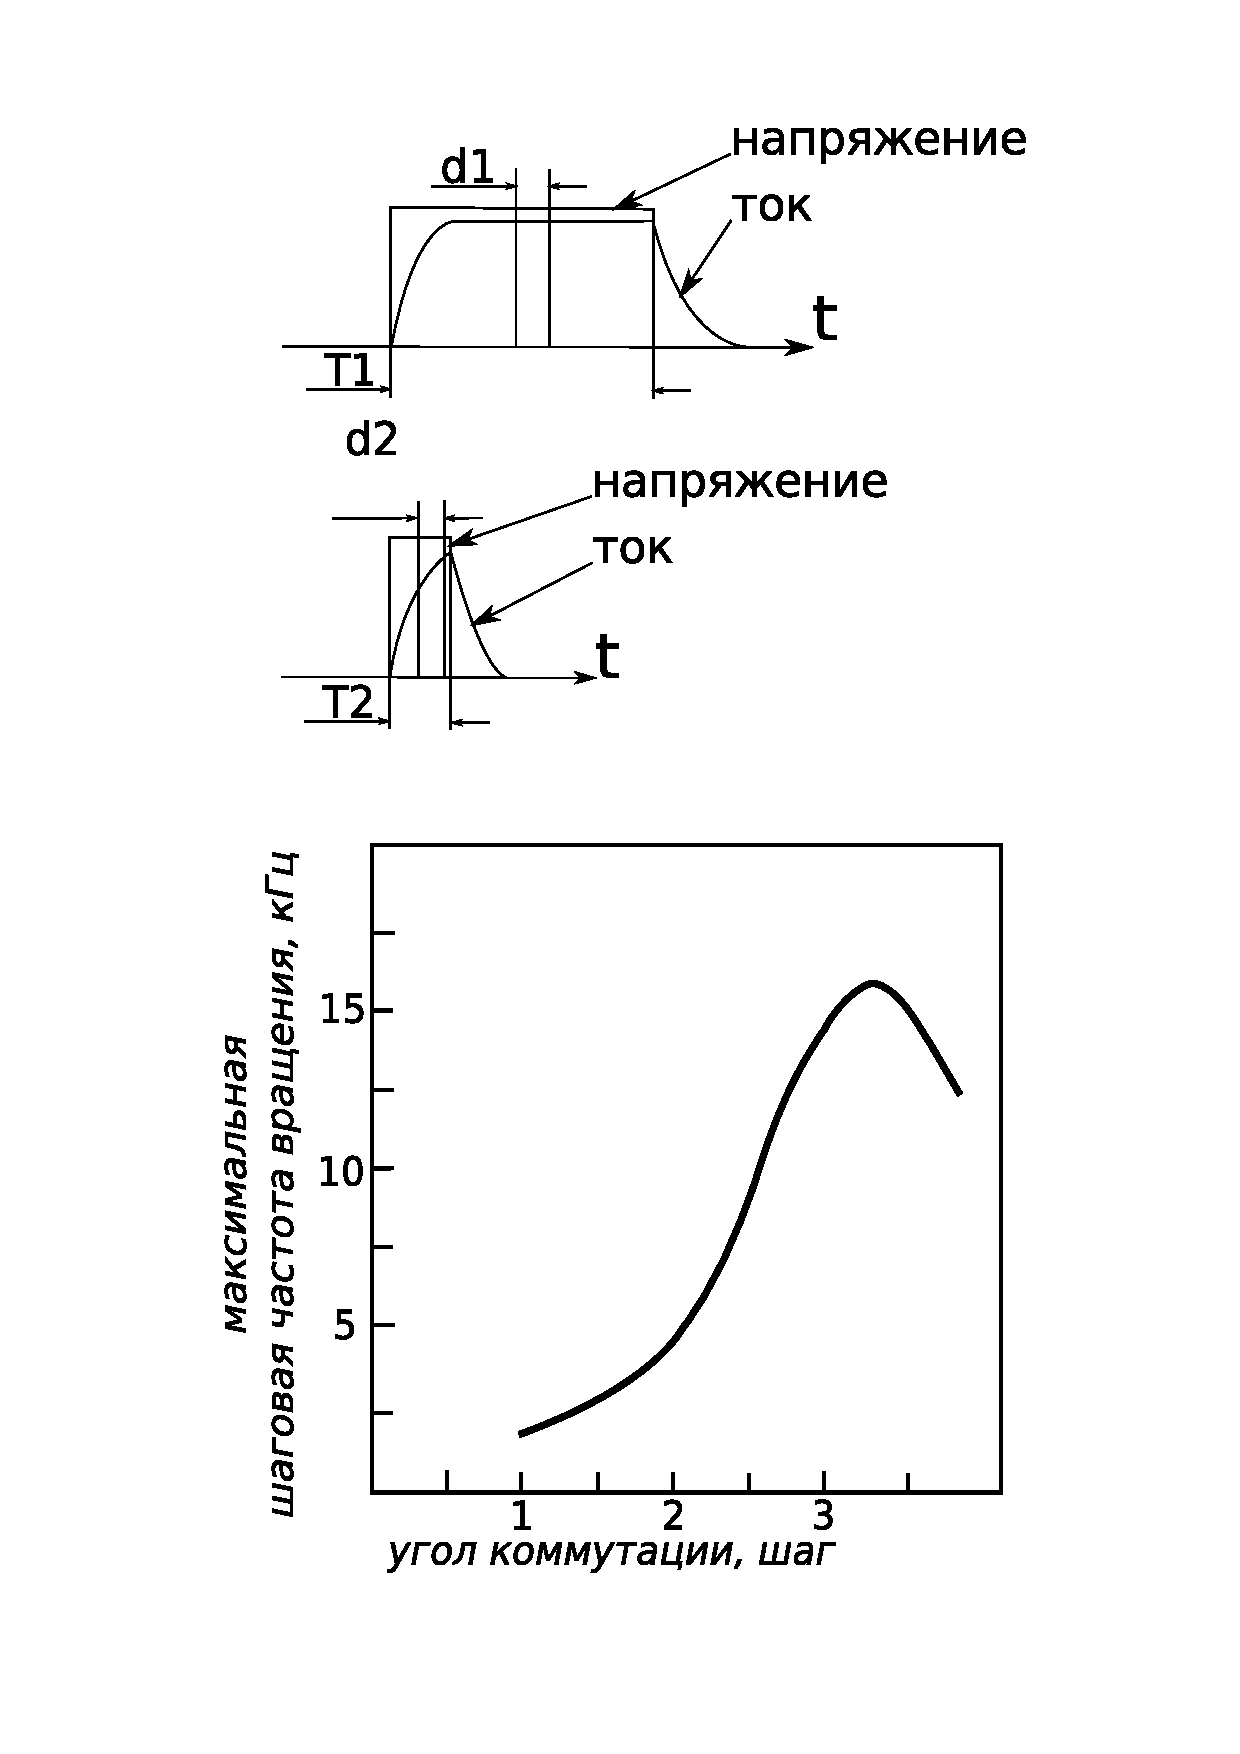
\includegraphics[width=\textwidth, keepaspectratio]{./src/pictures/max_step_motor_by_com_angle}
\caption{Влияние скорости на параметры управления}
\label{graph_speed_and_angle_comutation}
\end{figure}

Момент шагового двигателя в зависимости от угла отклонения ротора от положения равновесия:
\begin{equation}
    \label{torque_from_rotor_deviation}
    \tau = K_{T} I_{M} N_{r} ( \theta_{i} - \theta_{0} )
\end{equation}

$K_{T}$ - см. (\ref{torque_coeff})

$I_{M}$ - ток в обмотке, А

$N_{r} = 100$ - число зубцов ротора

$\theta_{0}$ - положение ровновесия, рад.

$\theta_{i}$ - текущее угловое положение, рад.
\newline
\newline

С помощью (\ref{torque_from_rotor_deviation}), задав желаемый угол коммутации и
средний (среднеинтегральный) момент, можно получить значение желаемого среднего
(среднеинтегрального) тока, необходимое для поддержания на данном шаге заданного момента.

Параметризуем угол коммутации и обозначим
$\theta_{com}$.
Согласно формуле (\ref{torque_from_rotor_deviation}) момент действующий на ротор
в начале импульса управления:

\begin{equation}
    \label{moment_to_rotor_at_the_begin_of_control_pulse}
    \tau_{begin} = K_{T} I_{M} N_{r} ( \theta_{com} )
\end{equation}

в конце импульса:

\begin{equation}
    \label{moment_to_rotor_at_the_end_of_control_pulse}
    \tau_{end} = K_{T} I_{M} N_{r} ( \theta_{com} - \theta_{s} )
\end{equation}

Средний момент для этого участка:
$$
    \tau_{step} = \frac{ \tau_{begin} + \tau_{end} }{ 2 }
$$
$$
    \tau_{step} = K_{T} I_{M} N_{r} ( \theta_{com} - \frac{ \theta_{s} }{ 2 } )
$$

